\documentclass[10pt]{article}

% EPS/PDF graphics
% Place figures in the Images directory in both the EPS and PDF
% formats, e.g., fig_1.eps and fig_1.pdf. Use the includegraphics
% command without file extension, e.g. \includegraphics*[width=3.25in]{fig_1}
% The pdflatex or latex programs then work automagically with the 
% appropriate formats.  EPS figures can be converted to PDF using
% the epstopdf program present on most Linux disributions
\usepackage{graphicx}

\begin{document}

\author{James N. Sturgis (james.sturgis@univ-amu.fr)}
\title{The RICS and NB program plugins for ImageJ.}

\maketitle

\section{Introduction}

This collection of plugins for the ImageJ analysis program implement Number and
Brightness analysis (N\&B) and Raster image Correlation Spectroscopy (RICS).

Why might you want these...

\subsection{Number and brightness analysis}

Brief introduction to theory and interest, with references.

\subsection{Raster image correlation analysis}

Brief introduction to theory and interest ICS and RICS to FCS.

\section{Installation}

To install the programs into Image J the RICS folder and its contents should 
be copied to the location where ImageJ looks for plugin programs. 

This varies on different operating systems, and can be modified at startup 
on the command line or by a startup script. 
A typical location on a Linux computer is ``(home)/.imagej/plugins''.
You can find the directory from within ImageJ. To find the plugin directory
follow the menu's ``Plugins$\rightarrow $ Utilities$\rightarrow $ ImageJ Properties'',
this will open a window with various informations including a line ``IJ.getDirectory("plugins")'',
you will probably have to scroll down the window to find it, in which the location of
the directory is given. Subdirectoies of this directory turn into sub-menus of the
``plugins'' menu.

Once the folder has been copied to the appropriate directory you will need to 
restart ImageJ, and that is all there is to it. 
You should now find in the ``Plugins'' menu a submenu ``RICS'' with
the items ``NB calculator'', ``RICS calculator'', ``RICS fit'' and ``RICS simulator'',
as shown in figure \ref{fig:MenuFig}.

\begin{figure}
\centerline{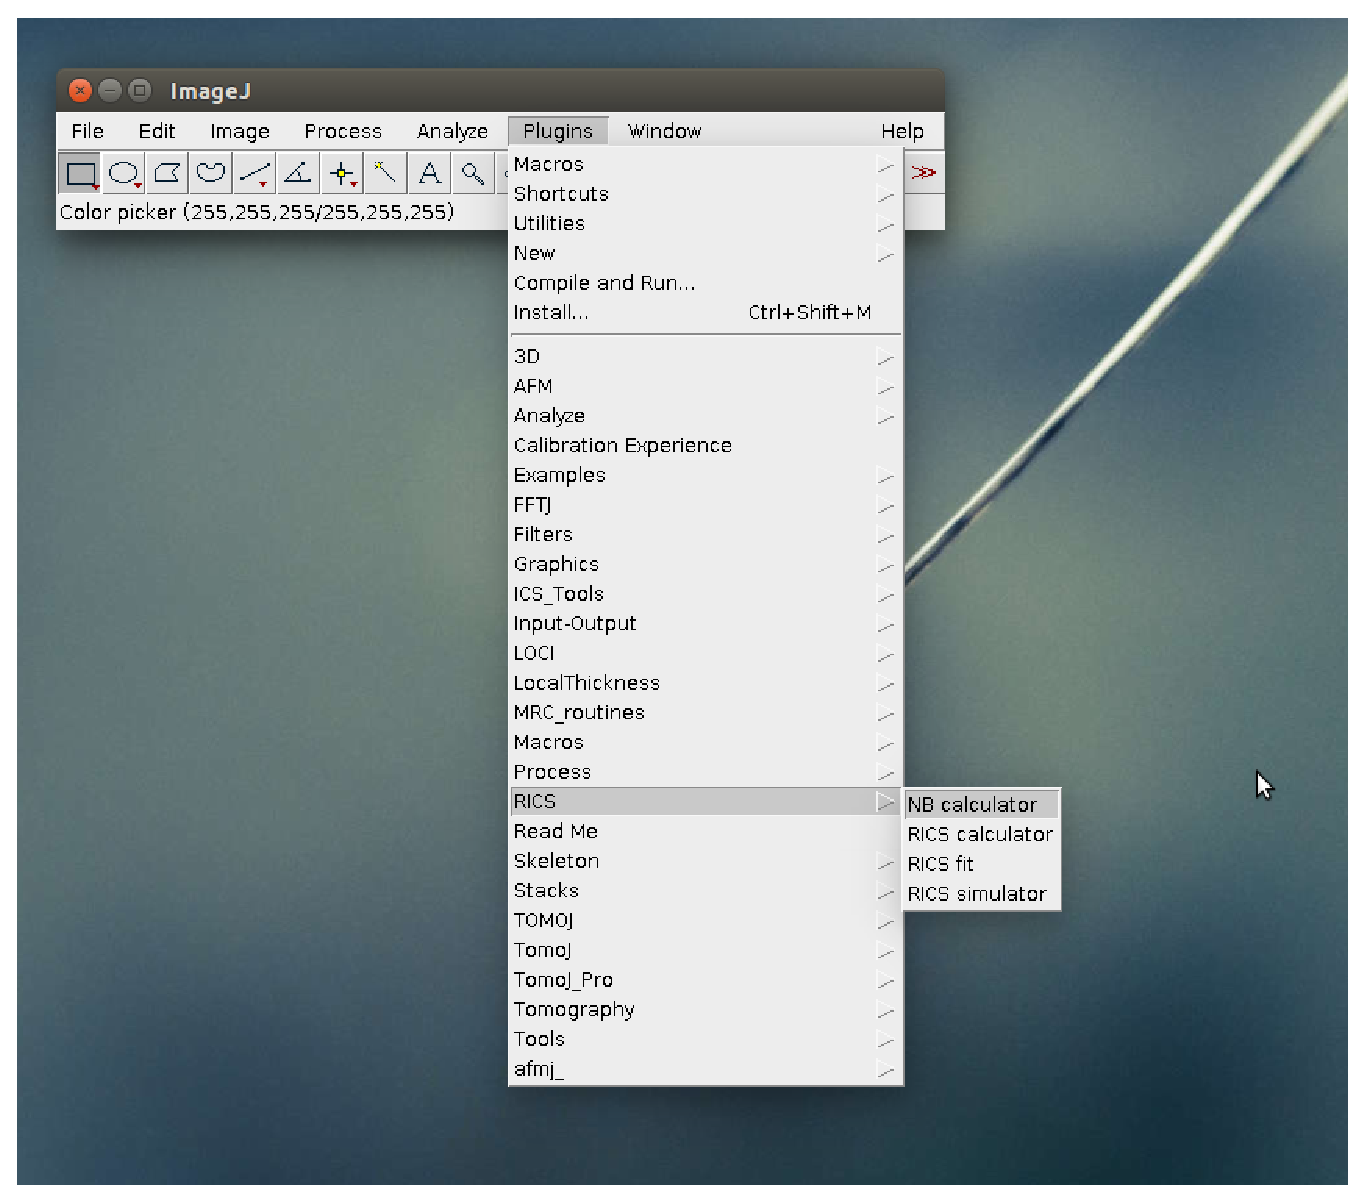
\includegraphics[width=.50\textwidth]{Images/MenuFig.eps}}
\caption{Screen capture showing RICS submenu of the plugin's menu in ImageJ on my computer.}
\label{fig:MenuFig}
\end{figure}

Strictly speaking it is only the ``.class'' files that need to be copied into the
plugins directory for ImageJ to recognise them and for you to be able to use them.
I however prefer to keep the files all together in a place where I might be able 
to find them again.
Unfortunately there is not a standard for incorporating documentation into the ImageJ
interface to give you access to the information in this file from the ImageJ 
user interface.

\section{Using the programs}

\subsection{General considerations}

The different programs are designed to operate on a images of a certain type and
acquired under appropriate conditions. So it is up to you to make sure the
images are appropriate for the analysis that you wish to perform. These points
are briefly discussed below. 

The RICS simulator is able to produce a stack of images appropriate for analysis
so I sigest you play with this to find out what conditions are appropriate for
your experiment. 

The optimum parameters for obtaining the images depend on the study 
and the microscope being used. However as the methods depend on analysing 
differences between the images and within the images thus the signal to noise ratio 
is often very low!!! This can be disconcerting for users who are used to trying to
obtain clear noise free images. Furthermore both methods can benefit from using
pixels smaller than the desired (obtainable) optical resolution, another suprise
for microscopists used to more standard techniques.

\subsection{Number and Brightness calculator}

This program requires a stack of images as input and then examines the differences
(noise) to extract information on the number and brightness of visible objects
in terms of number and brightness. The image is analysed pixel by pixel and so 
can distinguish different regions in the image.

The input image stack... what conditions give good results?

The output stack contains 6 images. These can be considered in pairs, first average 
of the different images in the stack (pixel by pixel), and the variance image 
which gives the variance of the intensity of each pixel. The next pair are Raw 
number and Raw brightness, these correspond to . Finally the last pair gives the 
number and brightness as analyzed pixel by pixel. In this pair of images for 
each pixel the observed intensity is considered to come from <number> objects of 
intensity <brightness>, it is thus the numberical values of the pixels which are 
important. The difference between the 'raw' values and the final values come from 
attempting to correct from detector shot noise.

In a future version of this software the analysis might go further to include
number vs brightness plots and the possibility of selecting regions based on the
number and brightness regime. If you are interested please let me know.

\subsection{RICS data simulation}

This program generates a stack of images corresponding that could be obtained 
from a particular homogeneous sample of diffusing fluorescent objects. This is 
useful to test if a particular analysis is likely to be productive and examine 
the influence of different parameters on the subsequent analysis.

\begin{figure}
\centerline{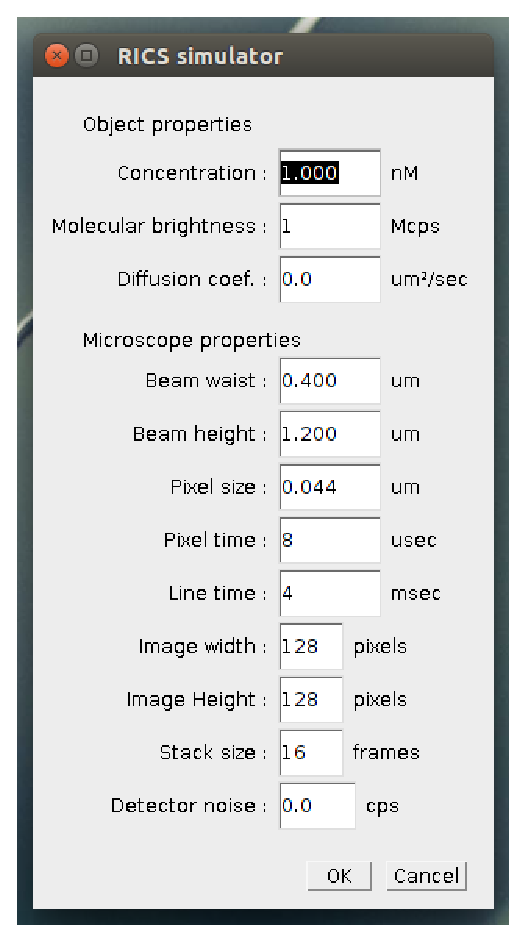
\includegraphics[width=.25\textwidth]{Images/MenuSimDialog.eps}}
\caption{Screen capture showing the RICS simulation dialog.}
\label{fig:MenuSimDialog}
\end{figure}

The program starts with a dialog box (figure \ref{fig:MenuSimDialog}) where the
user can set the different parameters concerning the sample parameters, the data 
acquisition parameters. 
The sample properties are: 
the concentration in nM, this controls how many objects are present; 
the molecular brightness in detected photons per $\mu $second (or millions of
    counts per second, Mcps), this influences the signal and visibility of the objects; 
the molecular diffusion coefficient in square microns per second, how fast the 
    objects move, diffusion is presumed normal in the three dimensions. 
The objects are probably beter behaved than most real samples as they never fade, 
never aggregate or stick to a surface!!!
The next set of parameters concerns the mircoscope settings for the virtual 
acquisition. First are the parameters of the instrument response function, this 
is taken as a three dimensional gaussian with a full width at half height in the 
x and y dimensions given by the beam waist and in the z dimension given by the 
beam height (both measurer in $\mu $m. This is clearly a simplification with 
respect to a real microscope as there is no astigmatism or distortion. 
The following parameters concern the scan parameters: 
the pixel size (in $\mu $m); 
the time per pixel (in $\mu $sec);
the time per line (in msec);
and the image size in pixels (the width is the number of pixels per line 
and height the number of lines per image). 
In this simulation the pixels are assumed to be square. 
Finally the number of independant images to simulate and the amount of random uncorrelated 
noise to add can be given. The default parameters correspond to a reasonable 
number of relatively bright objects that do not move.

Notice that the pixel size is well below the optical resolution. This is important for
RICS analysis as the analysis examines the distortion of the instrument point spread
function (PSF = optical resolution) by the movement of the particles so a good
measurement of the PSF requires significant over sampling.

Once the OK button is clicked a log window will open (if it is not already open)
to show how the simulation is progressing and the simulation will run calculating 
each frame separately, for each frame an entry in to log window will say how many particles are 
included in the simulation. 
Once all the simulations are performed the calculated image stack will be displayed (Figure \ref{fig:SimStack}). 
In the image on the left, for the default simulation, the objects are relatively round blobs since they are bright 
and stationary. 
Darker blobs correspond to those further from the focus and brighter one to those close to the focus.
In the image in the center the objects are moving at with a diffusion coefficient of 10 $\mu m^2 sec^{-1}$
and so appear as horizontal streaks, and this is exagerated in the right hand image of fast moving objects
500 $\mu m^2 sec^{-1}$.

\begin{figure}
\centerline{
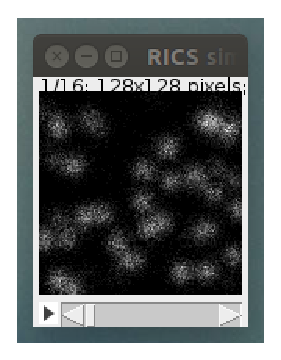
\includegraphics[width=.25\textwidth]{Images/SimStack1.eps}
\hskip 0.1\textwidth
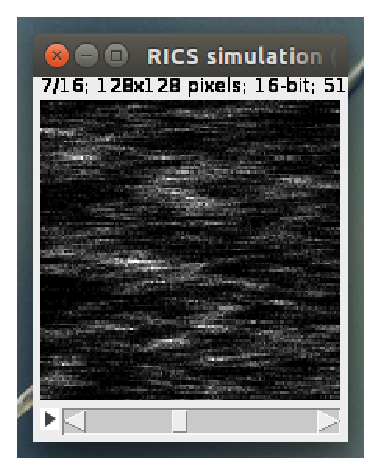
\includegraphics[width=.25\textwidth]{Images/SimStack2.eps}
\hskip 0.1\textwidth
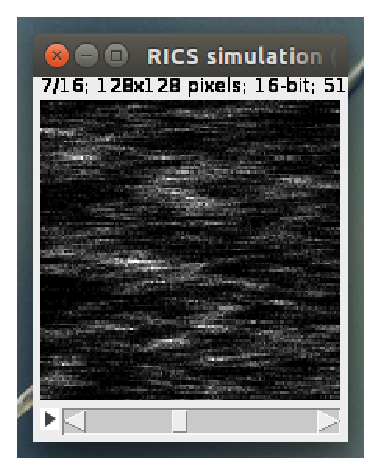
\includegraphics[width=.25\textwidth]{Images/SimStack2.eps}
}
\caption{Screen capture showing the result of the RICS simulation with 
(left) default parameters,
(center) faster moving particles (10 $\mu m^2 sec^{-1}$) in the presence of some detector noise,
(center) fast moving particles (500 $\mu m^2 sec^{-1}$).
}
\label{fig:SimStack}
\end{figure}

The simulation implementation constructs a simulation box of the image size in 
the x and y dimensions and 3 times the IRF height in the z dimension. In this 
box it places different particles and then overtime updates the particle 
positions and obtains the image. The algorithm, which could be improved, assumes 
periodic boundary conditions and no correlation between different frames.

\subsection{RICS data calculator}

This program calculates the spatial correlation function from a stack of images. 
There are no parameters to set or options, it performs a simple calculation and 
produces an image of the correlation function. This image is the point spread 
function (PSF), instrument response function (IRF), obtained from the analysis of 
the image, as distorted (or not) by the diffusion of the different objects. The 
resulting image is called shown in a new window and called ``Stack Correlation''.
The log window reports the average intensity of the series of images.

As can be seen in the figure \ref{fig:RICScalc}, the image for slowly moving objects, 
on the left, is essentially an undistorted psf while more rapidly diffusing objects,
right hand immage, give a psf that is shrunk in the vertical direction as objects 
move away after one or two lines.

The implementation is very simple running in real space. 
First the mean intensity is calculated, and then the normalized autocorrelation 
function is built up. Currently the correlation map is fixed at 33 x 33 pixels.
This size slightly restricts the degree of optical oversampling that can be used
to gain good results.

In a future version of this program it may be possible to change the size of the
correlation map. If you wish for this or other modifications please let me know.

\begin{figure}
\centerline{
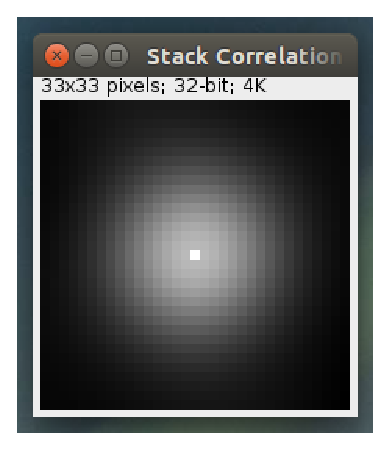
\includegraphics[width=.25\textwidth]{Images/RICScalc1.eps}
\hskip 0.1\textwidth
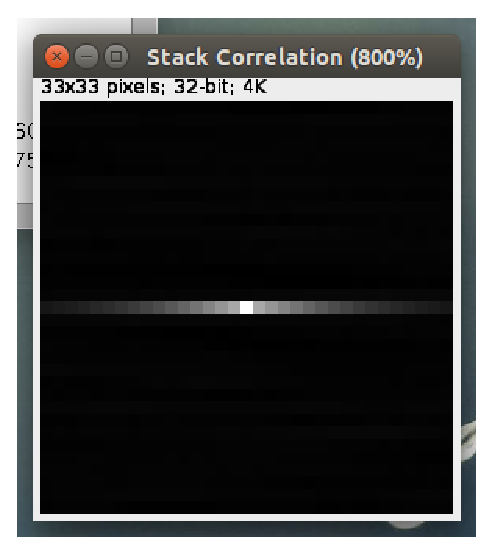
\includegraphics[width=.25\textwidth]{Images/RICScalc2.eps}
}
\caption{Screen capture showing the result of the RICS calculation with 
the simulation results:
(left) default parameters,
(center) fast moving particles (500 $\mu m^2 sec^{-1}$).
}
\label{fig:RICScalc}
\end{figure}

\subsection{RICS model fitting}

This program attempts to adjust a theoretical description of the autocorrelation 
function, to reflect the image provided. For example the autocorrelation function
produced by RICS calculator. The parameters of the fit can in turn be used to 
estimate the brightness and diffusion characteristics of the objects in the images
used to construct the autocorrelation function and the beam-waist of the PSF.

When the program is started a dialog opens to allow the user to enter: the data
acquisition parameters; initial estimations for adjustable parameters and
describe the calculation to perform (Figure \ref{fig:MenuFitDialog}).

\begin{figure}
\centerline{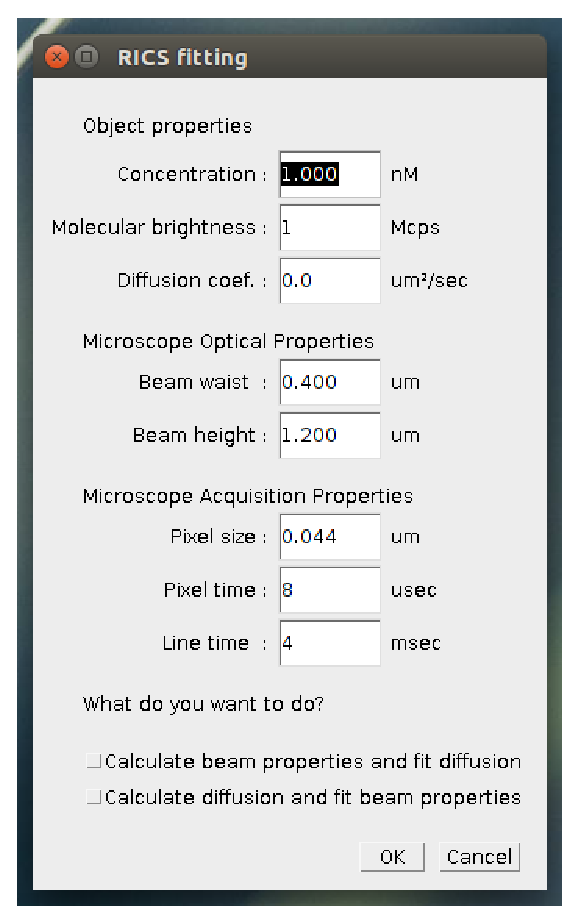
\includegraphics[width=.25\textwidth]{Images/MenuFitDialog.eps}}
\caption{Screen capture showing the RICS fitting dialog.}
\label{fig:MenuFitDialog}
\end{figure}

The program can be used in different ways: first, to calculate a theoretical 
autocorrelation function; second, to determine the beam waist from an
autocorrelation function of objects with a known diffusion constant; and third,
to calculate the diffusion constant if the beam geometry is known. The function
performed depends on the boxes checked at the bottom of the dialog: if no
boxes are checked the calculation is performed, if the boxes are checked either
the diffusion of beam properties are adjusted as appropriate.

The user should always provide the information for the scanning parameters: 
pixel size, pixel time and line time. These values define the x/y scale and the 
time scale implied by distortions of the PSF.
The user should also provide estimates, even if fitting, of the beam geometry. 
Note the ratio of the beam height to width is not adjusted and always presumed to
be known, this is because it has little effect on the result, and so is hard to
adjust, but does enter into the equations.

To simply calculate a theoretical result the appropriate value for the diffusion
constant should also be entered. When OK is clicked the program will produce
three new images entitled ``PSF part'', ``FCS part'' and ``Residuals'' and write
into the log window some information, figure \ref{fig:FitOutput}. The ``Residuals''
window contains the difference between the calculated autocorrelation function
and the intitial function, in the log window the residual is the sum of squares of
the pixels in this image, which can be used to obtain an estimate of the quality
of the correspondance. The calculated autocorrelation function is presented as 2
parts the (distorted) PSF as ``PSF part'' and the ``FCS part'' which is a 2
dimensional representation of the FCS curve. The FCS curve is scaled by setting G(0)
to assure that sum of residuals is 0. This value of G(0) is related to the number
of molecules in the excitation volume.

\begin{figure}
\centerline{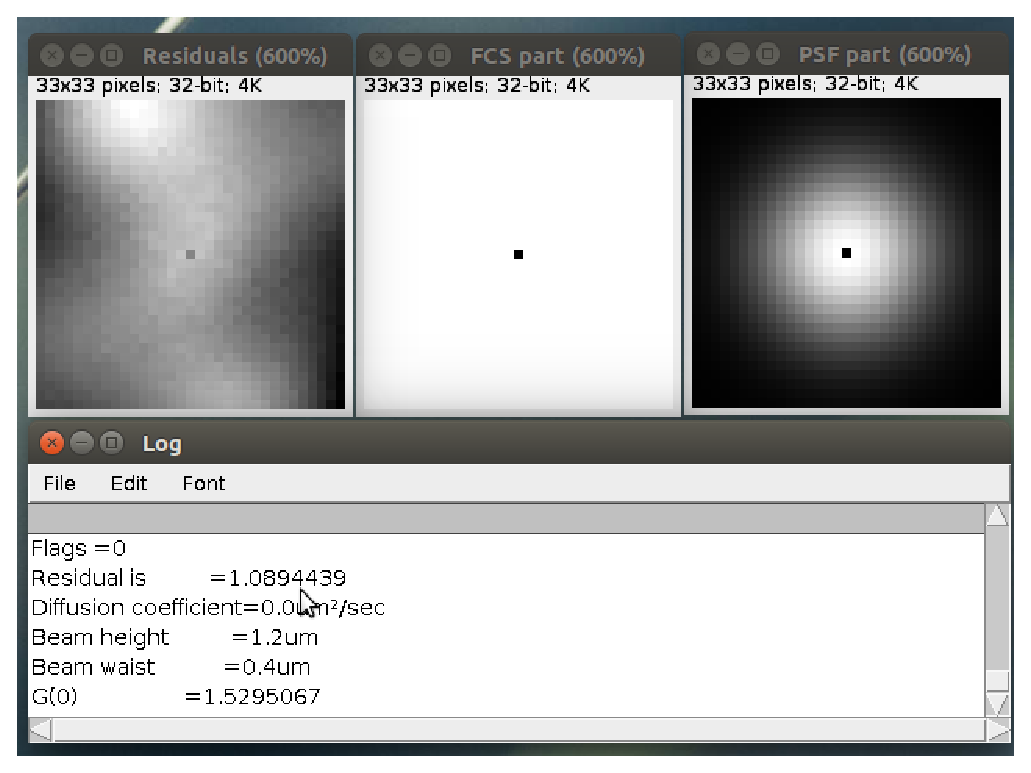
\includegraphics[width=.6\textwidth]{Images/FitOutput1.eps}}
\centerline{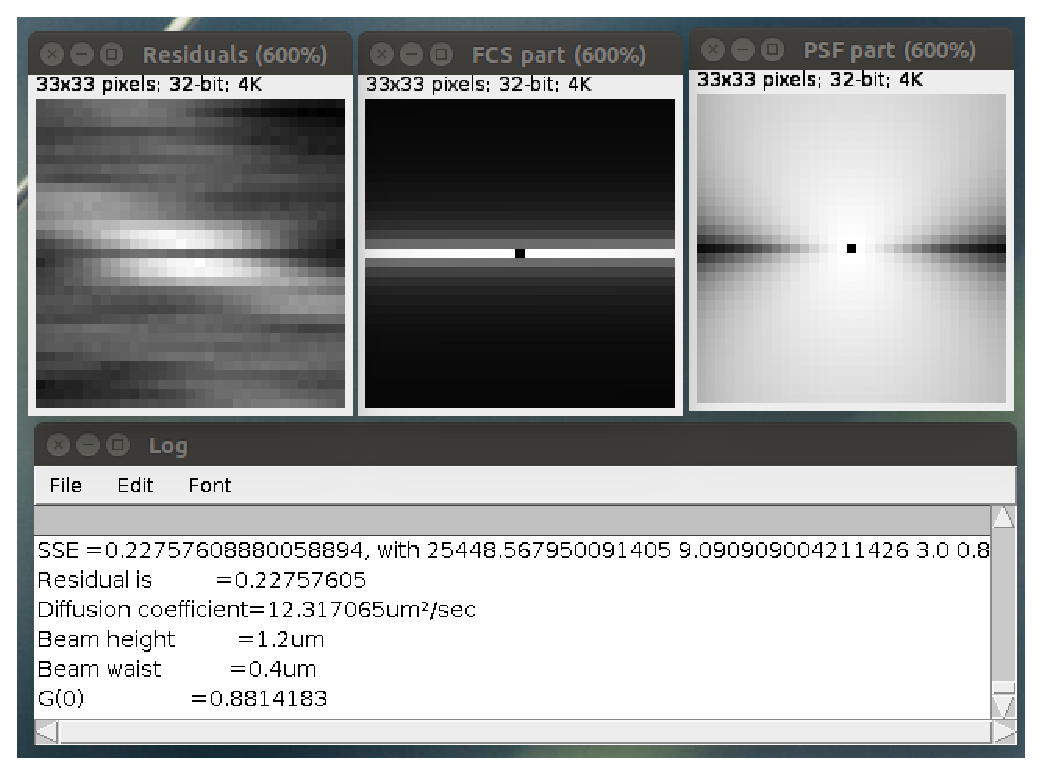
\includegraphics[width=.6\textwidth]{Images/FitOutput2.eps}}
\caption{Screen capture showing the RICS fitting output (top) calculation with
no object movement, (bottom) fitting with diffusion.}
\label{fig:FitOutput}
\end{figure}

To calculate the beam waist, the user should enter the molecule diffusion constant. 
The brightness and concentration are not important.
When OK is clicked the program will try to adjust the beam waist to get a good 
fit between a simulated PSF, a distorted two dimensional gaussian, and the 
observed autocorrelation function. In the log window will be reported information 
on the fit.

To calculate the diffusion coefficient the user should enter the beam waist 
information. The program will then adjust the simulated PSF and FCS curves to 
fit the autocorrelation function by modifying the diffusion coefficient. Information
ont the fit will be reported in the log window.

\end{document}
